\chapter{Solving the Equations of Motion}

\section{Static Solution}

\textcolor{red}{Static solution in context of bow: Bracing and equilibrium path, necessity for load control and displacement control}

A System with the equation of motion

\begin{align}
\boldsymbol{M}\,\ddot{\boldsymbol{u}} + \boldsymbol{q}(\boldsymbol{u},\,\dot{\boldsymbol{u}}) = \boldsymbol{p}
\end{align}

is in static equilibrium if~$\dot{\boldsymbol{u}},\,\ddot{\boldsymbol{u}} = \boldsymbol{0}$, leading to the static equilibrium condition

\begin{align}
\boldsymbol{q}(\boldsymbol{u},\,\boldsymbol{0}) = \boldsymbol{p}\label{eq:statics:equilibrium}
\end{align}

for the displacements $\boldsymbol{u}$ and the external loads $\boldsymbol{p}$.
This is a nonlinear system of equations and can be interpreted as the internal elastic forces~$\boldsymbol{q}$ being in balance with the external loads.

\subsection{The Basic Newton-Raphson Method}

Most frequently, when solving static problems, the external loads are given and the task is to calculate the corresponding equilibrium displacements.
Equation~(\ref{eq:statics:equilibrium}) is then a nonlinear system of equations in $\boldsymbol{u}$. Solving it can only be done numerically except for very simple examples.

An often used method for this kind of problem is the Newton-Raphson method. The basic idea behind it is to linearise the equilibrium equation~(\ref{eq:statics:equilibrium}) around a known displacement vector~$\boldsymbol{u}_i$ and solve the resulting linear equation to obtain an improved approximation~$\boldsymbol{u}_{i+1}$. Starting with an initial value~$\boldsymbol{u}_0$ the procedure is repeated until the solution is accurate enough by some convergence criterion.

Linearising of (\ref{eq:statics:equilibrium}) yields

\begin{align}
\boldsymbol{q}(\boldsymbol{u}_i) +
\underbrace{
\left(\frac{\partial \boldsymbol{q}}{\partial \boldsymbol{u}}\bigg \vert_{\boldsymbol{u}_i}\right)
}_{\boldsymbol{K}(\boldsymbol{u}_i)}
\underbrace{
(\boldsymbol{u}_{i+1} - \boldsymbol{u}_i)
}_{\Delta\boldsymbol{u}_i} &= \boldsymbol{p}
\end{align}

Solving for $\Delta\boldsymbol{u}_i$ leads to the iterative procedure

\begin{align}
\Delta\boldsymbol{u}_i &= \boldsymbol{K}^{-1}(\boldsymbol{u}_i)\left(\boldsymbol{p} - \boldsymbol{q}(\boldsymbol{u}_i)\right),\\
\boldsymbol{u}_{i+1} &= \boldsymbol{u}_i + \Delta\boldsymbol{u}_i.\label{eq:statics:newton_iteration}
\end{align}

In the implementation the tangent stiffness matrix is not actually inverted, because that's expensive and potentially inaccurate. Instead,~$\Delta\boldsymbol{u}_i$ is obtained by solving the equivalent linear system of equations using a decomposition of the stiffness matrix. The symmetry of the tangent stiffness can be used here. (It isn't necessarily positive definite though, like the stiffness matrices of linear mechanical systems.)

Convergence criteria are usually formulated in terms of change in displacement~$\Delta\boldsymbol{u}$, the residuum $\boldsymbol{p} - \boldsymbol{q}$ or their product $\Delta\boldsymbol{u}^\mathsf{T}(\boldsymbol{p}-\boldsymbol{q})$ (which has the dimension of an energy). We will use the energy criterion

\begin{equation*}
\Delta\boldsymbol{u}_{i}^\mathsf{T}(\boldsymbol{p}-\boldsymbol{q}(\boldsymbol{u}_i)) < \varepsilon
\end{equation*}

The basic Newton-Raphson method can be improved and extended in many ways, for example by combining it with a line search or by avoiding the calculation of the tangent stiffness matrix at every iteration (simplified Newton-Raphson method, BFGS method \textcolor{red}{[Source]}).

\subsection{Constrained Newton-Raphson method}

In the previous section the Newton-Raphson method was applied to the problem of calculating the equilibrium displacements of a system when all applied forces are known. This method is used in VirtualBow for finding the braced equilibrium state of the bow (see section \textcolor{red}{[Reference]}). However, when calculating the draw curve we don't actually know the draw forces, just the displacement of the string center. \textcolor{red}{Also: Load decrease.}

A solution to this is displacement control, where we prescribe a value for one of the displacement components and instead treat the corresponding external forces as a variable that is determined during solution.

The following derivation has been adapted from \cite{fem_script_uni_bochum}. Displacement control is a special case of a wider class of methods where the equilibrium equations are modified as
%
\begin{align}
\boldsymbol{q}(\boldsymbol{u}) - \lambda\,\boldsymbol{p} &= 0,\label{eq:equilibrium_dc}\\
c(\boldsymbol{u},\,\lambda) &= 0.\label{eq:constraint_dc}
\end{align}
%
Here the external forces are scaled by the unknown load factor $\lambda$. To compensate for this additional unknown, a scalar constraint~$c(\boldsymbol{u},\,\lambda) = 0$ on the displacements and the load parameter is introduced. Depending on the choice of constraint the method can be turned into load control, displacement control or other more sophisticated schemes like the arc-length method. We will carry out the derivation for the general case and specify the constraints later. This is also how these methods are implemented in VirtualBow: A general implementation for arbitrary constraints that is then specialized into load controlled and displacement controlled methods by providing the necessary constraints.

The system of nonlinear equations (\ref{eq:equilibrium_dc}), (\ref{eq:constraint_dc}) has to be solved for the displacements~$\boldsymbol{u}$ and the load parameter~$\lambda$. Like before, the Newton-Raphson method is used: The equations are linearised around a given approximation~$\{\boldsymbol{u}_i,\,\lambda_i\}$ and solved to obtain an improved approximiation~$\{\boldsymbol{u}_{i+1},\,\lambda_{i+1}\}$. This is repeated iteratively until displacements and load parameter satisfy the equilibrium equations~(\ref{eq:equilibrium_dc}) as well as the constraint equation~(\ref{eq:constraint_dc}) reasonably well as determined by some convergence criterion.

Carrying out the linearisation leads to the two equations
%
\begin{align}
\boldsymbol{q}(\boldsymbol{u}) - \lambda\,\boldsymbol{p}\:&\approx\:\boldsymbol{q}(\boldsymbol{u_{i}}) - \lambda_i\,\boldsymbol{p} + 
\underbrace{
\frac{\partial \boldsymbol{q}}{\partial \boldsymbol{u}}(\boldsymbol{u_{i}})
}_{\boldsymbol{K_{i}}}
\underbrace{
(\boldsymbol{u_{i+1}} - \boldsymbol{u_{i}})
}_{\Delta\boldsymbol{u_{i}}}
- \boldsymbol{p}
\underbrace{
\,(\lambda_{i+1} - \lambda_{i})
}_{\Delta \lambda_{i}}
\notag\\
&\approx\ \boldsymbol{q}(\boldsymbol{u_{i}}) - \lambda_i\,\boldsymbol{p} + \boldsymbol{K_{i}}\,\Delta\boldsymbol{u_{i}} - \boldsymbol{p}\,\Delta \lambda_{i}\label{eq:equilibrium_dc_lin}\\
\notag\\
c(\boldsymbol{u},\,\lambda) \ &\approx\ c(\boldsymbol{u_{i}},\,\lambda_{i}) + \frac{\partial c}{\partial \boldsymbol{u}}(\boldsymbol{u_{i}},\,\lambda_{i})(\boldsymbol{u_{i+1}} - \boldsymbol{u_{i}}) + \frac{\partial c}{\partial \lambda}(\boldsymbol{u_{i}},\,\lambda_{i})(\lambda_{i+1} - \lambda_{i})\notag\\
&\approx\ c(\boldsymbol{u_{i}},\,\lambda_{i}) + \frac{\partial c}{\partial \boldsymbol{u}}(\boldsymbol{u_{i}},\,\lambda_{i})\,\Delta\boldsymbol{u_{i}} + \frac{\partial c}{\partial \lambda}(\boldsymbol{u_{i}},\,\lambda_{i})\,\Delta \lambda_{i}\label{eq:constraints_dc_lin}
\end{align}

Equations~(\ref{eq:equilibrium_dc_lin}) and~(\ref{eq:constraints_dc_lin}) can written as the single linear system of equations
%
\begin{align}
\begin{bmatrix}
\boldsymbol{K_{i}} & -\boldsymbol{p}\\
\frac{\partial c}{\partial \boldsymbol{u}}(\boldsymbol{u_{i}},\,\lambda_{i}) & \frac{\partial c}{\partial \lambda}(\boldsymbol{u_{i}},\,\lambda_{i})
\end{bmatrix}
\begin{bmatrix}
\Delta\boldsymbol{u_{i}}\\
\Delta \lambda_{i}
\end{bmatrix}
=
\begin{bmatrix}
\lambda_i\,\boldsymbol{p} - \boldsymbol{q}(\boldsymbol{u_{i}})\\
-\boldsymbol{c}(\boldsymbol{u_{i}},\,f_{i})
\end{bmatrix}.\label{eq:total_dc_lin}
\end{align}
%
Solving this for the increments in displacement and load factor $\{\Delta\boldsymbol{u_{i}},\,\Delta \lambda_{i}\}$ allows us to calculate the next values as
%
\begin{align}
\boldsymbol{u_{i+1}} = \boldsymbol{u_{i}} + \Delta\boldsymbol{u_{i}}\\
\lambda_{i+1} = \lambda_{i} + \Delta \lambda_{i}.
\end{align}
%
However, directly solving~(\ref{eq:total_dc_lin}) is not  numerically efficient because the augmented stiffness matrix is no longer symmetric. A much better way to solve this is block elimination. We use the first row of~(\ref{eq:total_dc_lin}) to express~$\Delta\boldsymbol{u_{i}}$ as
%
\begin{align}
\Delta\boldsymbol{u_{i}} &= \boldsymbol{\alpha} + \boldsymbol{\beta}\,\Delta \lambda_{i}.\label{eq:auxiliary_disp_dc}
\end{align}
%
With the auxiliary vectors
%
\begin{align}
\boldsymbol{\alpha} &= \boldsymbol{K_{i}^{-1}}(\lambda_i\,\boldsymbol{p} - \boldsymbol{q}(\boldsymbol{u_{i}}))\label{eq:auxiliary_1}\\
\boldsymbol{\beta} &= \boldsymbol{K_{i}^{-1}}\,\boldsymbol{p}\label{eq:auxiliary_2}
\end{align}
%
These can be computed efficiently by exploiting the symmetry of the stiffness matrix $\boldsymbol{K_{i}}$.
%
To calculate $\Delta \lambda_i$, we substitute~(\ref{eq:auxiliary_disp_dc}) into the second row of~(\ref{eq:total_dc_lin}) which gives us
%
\begin{align}
&\frac{\partial c}{\partial \boldsymbol{u}}(\boldsymbol{u_{i}},\,\lambda_{i})\Delta\boldsymbol{u_{i}} + \frac{\partial c}{\partial \lambda}(\boldsymbol{u_{i}},\,\lambda_{i})\,\Delta \lambda_{i} = -c(\boldsymbol{u_{i}},\,\lambda_{i})\notag\\
&\frac{\partial c}{\partial \boldsymbol{u}}(\boldsymbol{u_{i}},\,\lambda_{i})(\boldsymbol{\alpha} + \boldsymbol{\beta}\,\Delta \lambda_{i}) + \frac{\partial c}{\partial \lambda}(\boldsymbol{u_{i}},\,\lambda_{i})\,\Delta \lambda_{i} = -c(\boldsymbol{u_{i}},\,\lambda_{i})\notag\\
&\ \ \vdots\notag\\
&\Delta \lambda_{i} = -\frac{c(\boldsymbol{u_{i}},\,\lambda_{i}) + \frac{\partial c}{\partial \boldsymbol{u}}(\boldsymbol{u_{i}},\,\lambda_{i})\,\boldsymbol{\alpha}}{\frac{\partial c}{\partial \boldsymbol{u}}(\boldsymbol{u_{i}},\,\lambda_{i})\,\boldsymbol{\beta} + \frac{\partial c}{\partial \lambda}(\boldsymbol{u_{i}},\,\lambda_{i})}.\label{eq:res_load_factor}
\end{align}

The Newton-Raphson iteration is now complete. To summarize: First, calculate $\boldsymbol{\alpha}$ and~$\boldsymbol{\beta}$ by solving~(\ref{eq:auxiliary_1}) and~(\ref{eq:auxiliary_2}). Then calculate the increment of the load parameter by using~(\ref{eq:res_load_factor}). The increment in displacements is then obtained by equation~(\ref{eq:auxiliary_disp_dc}).\\

\subsection{Constraints for load- and displacement control}

Finally, the constraint function and the parametrisation of the load vector have to be chosen. To get a displacement controlled method as initially stated we choose the constraint function as
%
\begin{align}
\boldsymbol{c}(\boldsymbol{u},\,\lambda) = u^{(k)} - \overline{u}
\end{align}
%
where~$u^k$ is the $k$-th component of the displacement vector that we want to control and $\overline{u}$ is the prescribed value for it. The partial derivatives are
%
\begin{align*}
\frac{\partial c}{\partial \boldsymbol{u}} &= \boldsymbol{e}_k,\quad
\frac{\partial c}{\partial \lambda} = 0,
\end{align*}
%
with $\boldsymbol{e}_k$ being the $k$-th unit vector. If a load controlled method is needed instead, the constraint becomes
%
\begin{align}
\boldsymbol{c}(\boldsymbol{u},\,\lambda) = \lambda - \overline{\lambda},
\end{align}
%
with the desired load factor $\overline{\lambda}$. Partial derivatives:
%
\begin{align*}
\frac{\partial c}{\partial \boldsymbol{u}} &= \boldsymbol{0},\quad
\frac{\partial c}{\partial \lambda} = 1,
\end{align*}

\subsection{Line search}

There is one last extension to the Newton-Raphson method that is needed for our purposes and that is line search. 

\textcolor{red}{Todo: Explain line search and why it helps with contact handling}

\newpage
\subsection{Finding the Braced Equilibrium State}

\textcolor{red}{Length of the string...}

\section{Dynamic Solution}

The equations of motion together with the initial displacements~$\boldsymbol{u}_0$ and velocities~$\boldsymbol{v}_0$ of the system form the second-order initial value problem

\begin{align}
\boldsymbol{M}\ddot{\boldsymbol{u}} &+ \boldsymbol{q}(\boldsymbol{u},\,\ddot{\boldsymbol{u}}) = \boldsymbol{p},\quad \boldsymbol{u}(0) = \boldsymbol{u}_0,\ \ddot{\boldsymbol{u}}(0) = \boldsymbol{v}_0.\label{eq:dynamics:system_equation}
\end{align}

for the displacements~$\boldsymbol{u}(t)$.

Numerical solution methods for initial value problems can be grouped into explicit and implicit ones.
Explicit methods use the current state of the system at time~$t$ to calculate the next state at~$t + \Delta t$.
Implicit methods instead find the next state by solving an equation that involves the current and the next state.
In the context of finite element analysis, implicit methods require equilibrium iterations at every time step involving the system's tangent stiffness matrix, while explicit methods only require simple vector operations.
Implicit methods therefore have a higher computational cost per step, but can make up for it by requiring less steps overall, as their better stability allows them to use much larger step sizes than explicit methods.

Explicit methods are easier to implement and are a good choice for small time scales, like impact and wave propagation problems.
They are most effective when the computation of the time steps is fast, so they work well with constant, diagonal (lumped) mass matrices and simple elements with low-order shape functions.

Implicit methods in contrast are well suited for larger time scales, where explicit algorithms would need too many steps.
Examples are structural response problems or numerically stiff systems, i.e. systems whose eigenfrequencies range from very small to very large.

VirtualBow currently uses the central difference method \cite{bib:dynamic_solution}, which is an explicit method often used in FEM.
Based on it's properties and the advantages of explicit methods it seems like a good choice.
However, implicit methods have not yet been tested with VirtualBow. The Newmark-beta method \textcolor{red}{Source} for example might be worth a try.

VirtualBow previously used the Runge-Kutta-Fehlberg-7-8 method provided by the \textcolor{red}{the odeint library}.
It performed worse than the central difference method, probably because of the high number of function evaluations carried out by an order~7/8 Runge-Kutta scheme.
The big advantage however was the timestep control based on error estimation, which meant that absolutely no user input regarding the timestep was necessary.

\subsection{The Central Difference Method}

The continuous solution $\boldsymbol{u}(t)$ is approximated by the discrete values~$\boldsymbol{u}_i = \boldsymbol{u}(t_{i})$ at the equidistant time steps~$t_i = i\cdot\Delta t$,\ \ $i \in \mathbb{N}$.
The acceleration~$\ddot{\boldsymbol{u}}_i$ can be approximated by a central difference quotient as

\begin{align}
\ddot{\boldsymbol{u}}_i &= \frac{\boldsymbol{u}_{i+1} - 2\,\boldsymbol{u}_{i} + \boldsymbol{u}_{i-1}}{\Delta t^2}\label{eq:dynamics:difference_acceleration}
\end{align}

Solving for~$\boldsymbol{u}_{i+1}$ and calculating the accelerations~$\ddot{\boldsymbol{u}}_{i}$ from the equation of motion~(\ref{eq:dynamics:system_equation}) leads to

\begin{align}
\boldsymbol{u}_{i+1} &= 2\,\boldsymbol{u}_{i} - \boldsymbol{u}_{i-1} + \Delta t^2\,\ddot{\boldsymbol{u}}_{i}\notag\\
&= 2\,\boldsymbol{u}_{i} - \boldsymbol{u}_{i-1} + \Delta t^2\,\boldsymbol{M}^{-1}(\boldsymbol{p}_i - \boldsymbol{q}_i).
\end{align}

This expression is already the core of the method, it allows the calculation of the next displacements~$\boldsymbol{u}_{i+1}$ from the current and previous system states.
It only involves cheap vector operations as the mass matrix is diagonal and doesn't have to be "actually" inverted.

Only the velocity is still missing. For this the central difference quotients of the displacements~$\boldsymbol{u}_{i+1}$,~$\boldsymbol{u}_{i}$ and~$\boldsymbol{u}_{i-1}$ are used to calculate the intermediate velocities

\begin{align}
\dot{\boldsymbol{u}}_{i+\frac{1}{2}} &= \frac{\boldsymbol{u}_{i+1} - \boldsymbol{u}_{i}}{\Delta t},\\
\dot{\boldsymbol{u}}_{i-\frac{1}{2}} &= \frac{\boldsymbol{u}_{i} - \boldsymbol{u}_{i-1}}{\Delta t}.
\end{align} 

The actual new velocity~$\dot{\boldsymbol{u}}_{i+1}$ is linearly extrapolated from those,

\begin{align}
\dot{\boldsymbol{u}}_{i+1} &= \dot{\boldsymbol{u}}_{i+\frac{1}{2}} + \frac{1}{2}\,\left(\dot{\boldsymbol{u}}_{i+\frac{1}{2}} - \dot{\boldsymbol{u}}_{i-\frac{1}{2}}\right),\notag\\
&= \frac{1}{\Delta t}\,\left(\frac{3}{2}\,\dot{\boldsymbol{u}}_{i+1} - 2\,\dot{\boldsymbol{u}}_{i} + \frac{1}{2}\,\dot{\boldsymbol{u}}_{i-1}\right).
\end{align}

This last step is actually a custom modification as far as I can tell.
All descriptions of the central difference method that I've seen end with the calculation of~$\dot{\boldsymbol{u}}_{i+\frac{1}{2}}$.

The initialisation of the procedure needs some special attention, as the method uses the previous displacements~$\boldsymbol{u}_{i-1}$ that don't exist yet at time~$t = 0$.
Instead,~$\boldsymbol{u}_{-1}$ is estimated by using finite difference approximations of the system's initial velocity and acceleration:

\begin{align}
\dot{\boldsymbol{u}}_0 &= \frac{\boldsymbol{u}_{1} - \boldsymbol{u}_{-1}}{2\,\Delta t},\\
\ddot{\boldsymbol{u}}_0 &= \frac{\boldsymbol{u}_{1} - 2\,\boldsymbol{u}_{0} + \boldsymbol{u}_{-1}}{\Delta t^2},\\
&\Rightarrow \boldsymbol{u}_{-1} = \boldsymbol{u}_{0} - \Delta t\,\dot{\boldsymbol{u}}_{0} + \frac{\Delta t^2}{2}\,\ddot{\boldsymbol{u}}_{0}.
\end{align}

A last but very important question is how to choose the timestep~$\Delta t$.
The timestep influences the computational effort, the accuracy of the solution but most importantly the stability of the algorithm.
A too large time step will lead to a solution that "explodes" numerically.
For linear, conservative mechanical systems of the form

\begin{align}
\boldsymbol{M}\ddot{\boldsymbol{u}} + \boldsymbol{K}\boldsymbol{u} = \boldsymbol{p}
\end{align}

the stability condition is

\begin{align}
\Delta t \le \frac{2}{\omega_{max}}\label{eq:timestep_bound}
\end{align}

where~$\omega_{max}$ is the maximum natural frequency \cite{bib:dynamic_solution} of the system.
Unfortunately there is no such analytical bound on~$\Delta t$ that guarantees stability for nonlinear systems.
A common thing to do is to linearise the system around the current configuration and apply (\ref{eq:timestep_bound}) anyway.
A safety factor~$0 < \beta < 1$ is introduced to account for the uncertainties and the timestep is set to

\begin{align}
\Delta t = \beta \frac{2}{\omega_{max}}.
\end{align}

This doesn't guarantee stability in a strict sense, but it's okay for practical purposes. A common choice is~$\beta = 0.9$ but VirtualBow uses a lower value for the sake of robustness. The frequency $\omega_{max}$ is sometimes estimated by using the bound

\begin{align}
\omega_{max} \le \max_{i}\,\{\omega_{max,\,i}\}
\end{align}

where $\omega_{max,\,i}$ is the maximum natural frequency of the respective finite element~$i$. But this leads to larger time steps than necessary and actually causes more implementation effort than just solving the generalised eigenvalue problem

\begin{align}
\left(\boldsymbol{M} - \omega^2\boldsymbol{K}\right)\boldsymbol{\bar{u}} = 0\label{eq:natural_frequencies}
\end{align}

which is what VirtualBow does.

\textcolor{red}{No damping here. For a version with damping see the LS-Dyna theoretical manual of 2006.}

\subsection{Stopping Criterion and Progress Estimation}

Everything has to stop at some point, even the dynamic simulation. But when exactly?
The simulated time interval has to include the separation of the arrow from the bow plus some additional time, because some interesting things like e.g. the maximum force on the string only happen after the arrow left the bow.
A related requirement is that there needs to be some estimation for the simulation progress that can be shown the user.
But how can the progress be estimated even though the ending time of the simulation isn't known in advance?

The current approach is to simulate the time interval~$[0,\,\alpha\,T]$ where~$T$ is the (yet unknown) time for the arrow to reach brace height and~$\alpha$ is an arbitrary positive factor.
The default value is~$\alpha = 1.5$. The simulation progress at time~$\overline{t}$ can now be formally written as

\begin{equation}
\rm{progress} = \frac{\overline{t}}{\alpha\,T}\cdot 100\%.\label{eq:solution:progress}
\end{equation}

But only formally, because~$T$ is unknown as long as~$\overline{t} < T$, i.e. as long as the arrow has not yet actually reached brace height. For this first part of the simulation~$T$ is estimated by using the current time~$\overline{t}$ and position~$\overline{u}$ of the arrow and extrapolate to the time when the arrow will reach brace height.

\begin{figure}[h]
\centering
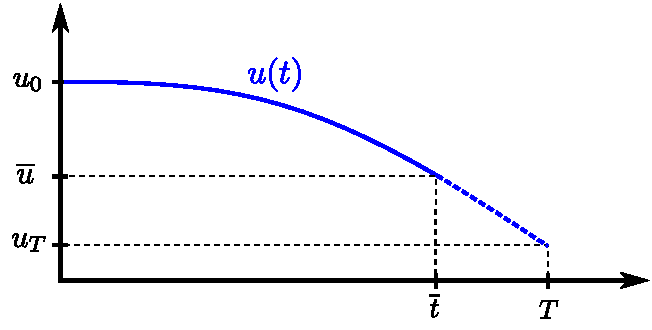
\includegraphics[width=0.8\textwidth]{figures/solution/dynamic_progress}
\caption{Arrow position $u(t)$ during the shot}
\label{fig:solution:dynamic_progress}
\end{figure}

The progression of the arrow position, denoted by~$u(t)$, typically looks like shown in figure~\ref{fig:solution:dynamic_progress}.
It starts at time~$t = 0$ at full draw~$u_0$ and reaches brace height~$u_T$ at the time~$t = T$ by definition.
If the draw curve of the bow is assumed to be approximately linear then~$u(t)$ will resemble the cosine quarter-wave

\begin{equation}
u(t) \approx u_{0}\,\cos{\left(C\,t\right)}.\label{eq:solution:progress:ansatz}
\end{equation}

Not all draw curves might be approximately linear, but this is only about crude progess estimation after all.
The constant~$C$ is obtained by applying equation~(\ref{eq:solution:progress:ansatz}) to the current time and position,

\begin{equation}
u(\overline{t}) = \overline{u} \Rightarrow \ C = \frac{1}{\overline{t}}\,\arccos{\left(\frac{\overline{u}}{u_0}\right)}.\label{eq:solution:progress:constant}
\end{equation}

Now $T$ can be extrapolated from~(\ref{eq:solution:progress:ansatz}) using the condition~$u(T) = u_T$,

\begin{align}
T = \frac{1}{C}\,\arccos{\left(\frac{u_T}{u_0}\right)} = \overline{t}\ \frac{\arccos{\left(\nicefrac{u_T}{u_0}\right)}}{\arccos{\left(\nicefrac{\overline{u}}{u_0}\right)}}.
\end{align}

This approximation for~$T$ is used in the progress estimation~(\ref{eq:solution:progress}) until the arrow has reached brace height. Then the actual value is known and used for the rest of the simulation.




\newpage
\section{Model setup}

\subsection{Finding the damping parameters}

The damping parameter $\eta A$ of the string is determined analytically such that the damping ratio associated with the first (longitudinal) natural frequency matches the user supplied value. From Appendix \ref{chapter:viscoelastic-bar-vibrations} it follows that
%
\begin{equation}
\eta A = \frac{4L}{\pi}\,\sqrt{\rho A\,EA}\,\zeta
\end{equation}

in order for this to be true, where $L$ is half the total length of the string to match the boundary conditions used.

\subsection{Distributing string elements}

\begin{figure}[h]
\centering
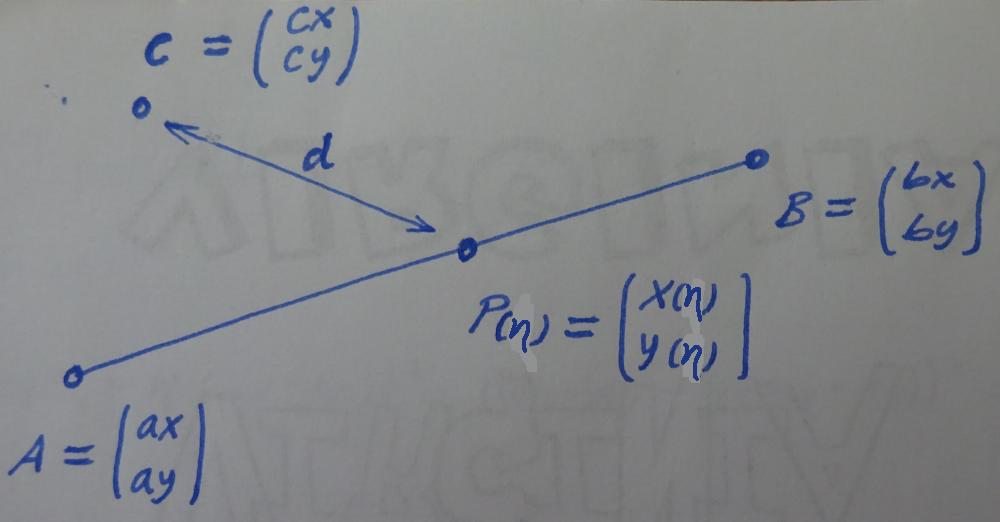
\includegraphics[width=0.8\textwidth]{figures/setup/line-distance}
\caption{Problem}
\label{fig:solution:dynamic_progress}
\end{figure}

Problem: Find a point $P$ on the line between $A$ and $B$ which has the euclidean distance $d$ to point $C$.

Parametrisation of the points $P$:

\begin{align*}
P(\eta) &= A + \eta\,(B-A),\quad \eta \in [0,\,1]
\end{align*}

Distance condition:

\begin{align*}
&\lVert C - P(\eta)\rVert = d\\
\Leftrightarrow\:&\lVert
\begin{bmatrix}
c_x - a_x - \eta\,(b_x - a_x) \\ c_y - a_y - \eta\,(b_y - a_y)
\end{bmatrix}
\rVert = d\\
\Leftrightarrow\:&\left(c_x - a_x - \eta\,(b_x - a_x)\right)^2 + \left(c_y - a_y - \eta\,(b_y - a_y)\right)^2 = d^2\\
\Leftrightarrow\:&\left((b_x - a_x)^2 + (b_y - a_y)^2\right)\,\eta^2-2\left((c_x - a_x)(b_x - a_x) + (c_y - a_y)(b_y - a_y)\right)\,\eta\\
&+(c_x - a_x)^2 + (c_y - a_y)^2 - d^2 = 0
\end{align*}

This is a quadratic equation for $\eta$. Take smallest solution in $[0,\,1]$.
